%\documentclass[12pt]{oblivoir}
\documentclass[12pt]{article}
\usepackage{kotex}
\usepackage{graphicx}
\setlength{\parskip}{6pt}   % 단락사이 빈여백 공간설정.
\setlength{\parindent}{0pt} % 단락사이 들여쓰기 않함.

\begin{document}

\textbf{GUI와 CLI 전쟁}

\bigskip

매우 단순한 \LaTeX\/ 문서로 \LaTeX\/을 사용하여 문서를 작성합니다.


\section{초록}

GUI 종족과 CLI 종족간의 전쟁은 끝이 보이지 않고 있다.
두 종족간의 전쟁은 윈도우의 출현으로 GUI 종족의 일방적인 승리로 끝날 것으로 보였지만, 클라우드 시대의 출현으로 다시 CLI 종족이 주도권을 잡아가고 있는 모양이 되었다.
CLI 종족은 과거 소수였지만, 소프트웨어 카펜트리\cite{DBLP:journals/corr/SimperlerW15}를 내세워서 GUI 종족을 흡수하면서 세력을 급격히 확장시키고 있다.

두 종족간의 전쟁은 어떻게 전개될까? 과연 과학 컴퓨팅\cite{10.1371/journal.pbio.1001745}는 도움이 될까?

\begin{itemize}
  \item 한글 사용이 가능한지 확인합니다.
  \item 수식 사용이 가능한지 확인합니다.
  \item 표 사용이 가능한지 확인합니다.
  \item 그림 사용이 가능한지 확인합니다.
  \item 참고문헌 사용이 가능한지 확인합니다.
\end{itemize}


\section{ 종족전쟁 도해}

\begin{figure} [!htb]
  \centerline{
\includegraphics[width=\textwidth]{fig/gui-vs-cli.jpg}}
\end{figure}

\section{수식}

$생산성 = \frac{CLI^2}{GUI}$

\section{그림}

첫번째 그림:

\centerline{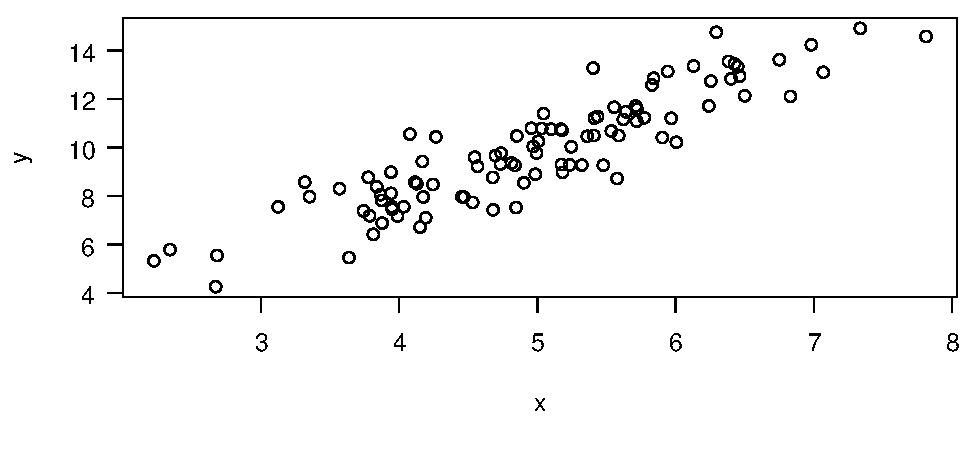
\includegraphics[width=\textwidth]{fig/fig1.pdf}}

두번째 그림:

\centerline{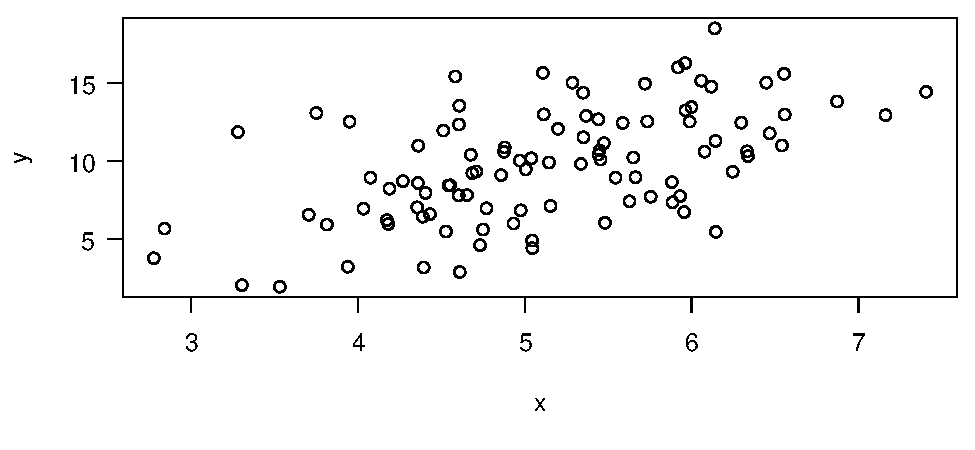
\includegraphics[width=\textwidth]{fig/fig2.pdf}}

\section{참고문헌}

% Insert bibliography
\bibliography{data_science}{}
\bibliographystyle{plain}


\end{document}